\documentclass[12pt]{article}
\usepackage[utf8]{inputenc}

\usepackage{lmodern}

\usepackage{enumitem}
\usepackage[margin=2cm]{geometry}

\usepackage{amsmath, amsfonts, amssymb}
\usepackage{graphicx}
\usepackage{tikz}
\usepackage{pgfplots}
\usepackage{multicol}

\usepackage{comment}
\usepackage{url}
\usepackage{calc}
\usepackage{subcaption}

\usepackage{array}
\usepackage{blkarray,booktabs, bigstrut}

\pgfplotsset{compat=1.16}

% MATH commands
\newcommand{\ga}{\left\langle}
\newcommand{\da}{\right\rangle}
\newcommand{\oa}{\left\lbrace}
\newcommand{\fa}{\right\rbrace}
\newcommand{\oc}{\left[}
\newcommand{\fc}{\right]}
\newcommand{\op}{\left(}
\newcommand{\fp}{\right)}

\newcommand{\bi}{\mathbf{i}}
\newcommand{\bj}{\mathbf{j}}
\newcommand{\bk}{\mathbf{k}}
\newcommand{\bF}{\mathbf{F}}

\newcommand{\mR}{\mathbb{R}}

\newcommand{\ra}{\rightarrow}
\newcommand{\Ra}{\Rightarrow}

\newcommand{\sech}{\mathrm{sech}\,}
\newcommand{\csch}{\mathrm{csch}\,}
\newcommand{\curl}{\mathrm{curl}\,}
\newcommand{\dive}{\mathrm{div}\,}

\newcommand{\ve}{\varepsilon}
\newcommand{\spc}{\vspace*{0.5cm}}

\DeclareMathOperator{\Ran}{Ran}
\DeclareMathOperator{\Dom}{Dom}

\newcommand{\exo}[3]{\noindent\textcolor{red}{\fbox{\textbf{Section {#1} | Problem {#2} | {#3} points}}}\\}

\begin{document}
	\noindent \hrulefill \\
	MATH-302 \hfill Pierre-Olivier Paris{\'e}\\
	Proof of $\lim_{x \ra 0} \sin x / x = 1$ \hfill Fall 2022\\\vspace*{-0.7cm}
	
	\noindent\hrulefill
	
	\spc
	
	We will prove that
		\begin{align*}
		\lim_{x \ra 0} \frac{\sin x}{x} = 1 .
		\end{align*}
		
	To prove that, we will use the Squeeze Theorem. Therefore, we need to ``squeeze'' the function $f(x) = \frac{\sin x}{x}$ between two functions $h$ and $g$ such that $h(x) \leq f(x) \leq g(x)$ and
		\begin{align*}
		\lim_{x \ra 0} h(x) = 1 \quad \text{ and } \quad \lim_{x \ra 0} g(x) = 1 .
		\end{align*}
	
	To find $g(x)$ and $h(x)$, let's consider the following geometric construction:
		\begin{center}
		\centering
		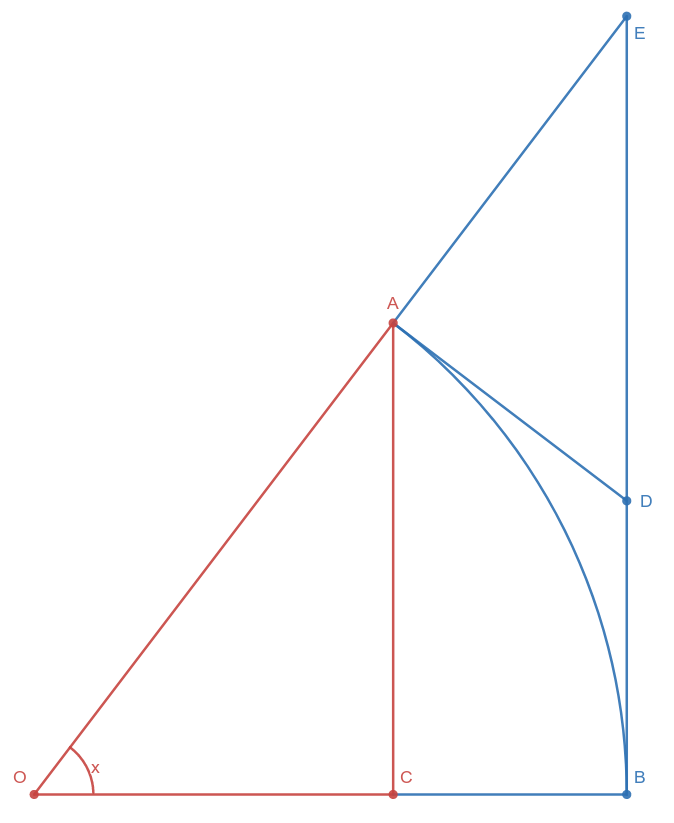
\includegraphics[scale=0.25]{Screenshot-from-2022-08-24 22-31-46.png}
		\end{center}
	In red, we have a right triangle $\vartriangle OAC$ with an angle at $O$ of $x$ and a right angle at $C$. In blue, we have another right triangle $\vartriangle OBE$ with an angle at $O$ of $x$ and a right angle at $B$. The length of the segment $OA$ is $1$ and the length of the segment $OB$ is also $1$. 
	
	First of all, we see that the length of the segment $CA$ is $\sin x$ and the length of the arc $BA$ is $x$. We also see that the length of the arc $BA$ is greater that the length of the segment $CA$. Therefore, we get
		\begin{align*}
		\sin x \leq x \quad \Rightarrow \quad \frac{\sin x}{x} \leq 1 .
		\end{align*}
	We let $g(x) = 1$.
	
	Second of all, we see that the segment $AD$ is perpendicular to the segment $OE$. Also, the length of the arc $BA$ is smaller than the sum of the length of the segments $BD$ and the length of the segment $DA$. Moreover, the triangle $\vartriangle ADE$ has a right angle at $A$ and its hypothenus is the segment $DE$. This means that the length of the segment $DA$ is smaller than the length of the segment $DE$. We then get
		\begin{align*}
		x \leq \overline{BD} + \overline{DA} \leq \overline{BD} + \overline{DE} = \overline{BE} .
		\end{align*}
	However, by the definition of the tangent of $x$, we have
		\begin{align*}
		\tan x = \frac{\overline{BE}}{\overline{OB}} = \overline{BE}
		\end{align*}
	where the last equality comes from the fact that $\overline{OB} = 1$. Therefore, we get
		\begin{align*}
		x \leq \overline{BE} = \tan x
		\end{align*}
	and since $\tan x = \sin x / \cos x$, this last inequality implies that
		\begin{align*}
		x \leq \frac{\sin x }{\cos x} \quad \Rightarrow \quad \cos x \leq \frac{\sin x}{x} .
		\end{align*}
	So let $h (x) = \cos (x)$.
	
	Finally, we see that 
		\begin{align*}
		\lim_{x \ra 0} \cos x = 1 = \lim_{x \ra 0} 1 .
		\end{align*}
	Since $\cos x \leq \frac{\sin x}{x} \leq 1$, by the Squeeze Theorem, we conclude that
		\begin{align*}
		\lim_{x \ra 0} \frac{\sin x}{x} = 1 .
		\end{align*}
\end{document}